\documentclass[tikz,border=10pt]{standalone}
\usepackage[T1]{fontenc}
\usepackage{lmodern,amsmath,amssymb}
\usetikzlibrary{arrows.meta,positioning}
\definecolor{ink}{HTML}{183444}
\definecolor{blue}{HTML}{1B6780}
\definecolor{amber}{HTML}{AD601A}
\begin{document}
\hyphenpenalty=10000\exhyphenpenalty=10000
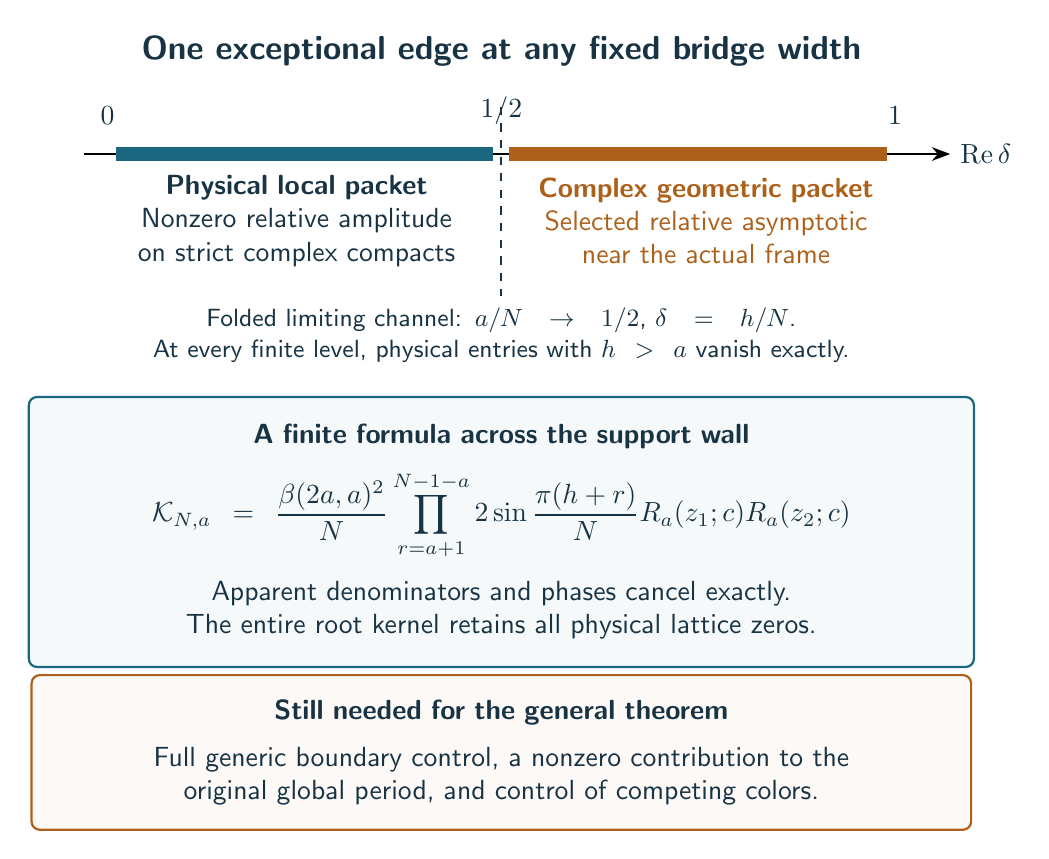
\begin{tikzpicture}[font=\sffamily,text=ink,>=Stealth]
 \node[font=\sffamily\large\bfseries] at (5,1.3)
 {One exceptional edge at any fixed bridge width};
 \draw[->,thick] (-.3,0)--(10.7,0) node[right] {$\operatorname{Re}\delta$};
 \draw[line width=5pt,blue] (.1,0)--(4.9,0);
 \draw[line width=5pt,amber] (5.1,0)--(9.9,0);
 \draw[dashed,thick,ink] (5,.6)--(5,-1.8);
 \foreach \x/\label in {0/0,5/{1/2},10/1}
   \node[above=7pt] at (\x,0) {$\label$};
 \node[align=center,text width=4.4cm] at (2.4,-.85)
 {\textbf{Physical local packet}\\Nonzero relative amplitude\\on strict complex compacts};
 \node[align=center,text width=4.4cm,text=amber] at (7.6,-.85)
 {\textbf{Complex geometric packet}\\Selected relative asymptotic\\near the actual frame};
 \node[align=center,text width=11cm,font=\sffamily\small] at (5,-2.3)
 {Folded limiting channel: $a/N\to1/2$, $\delta=h/N$.\\
 At every finite level, physical entries with $h>a$ vanish exactly.};
 \node[draw=blue,thick,rounded corners=3pt,fill=blue!4,
       text width=11.3cm,align=center,inner sep=10pt] at (5,-4.8)
 {\textbf{A finite formula across the support wall}\\[7pt]
 $\displaystyle \mathcal K_{N,a}
 =\frac{\beta(2a,a)^2}{N}
   \prod_{r=a+1}^{N-1-a}2\sin\frac{\pi(h+r)}{N}
   R_a(z_1;c)R_a(z_2;c)$\\[7pt]
 Apparent denominators and phases cancel exactly.\\
 The entire root kernel retains all physical lattice zeros.};
 \node[draw=amber,thick,rounded corners=3pt,fill=amber!4,
       text width=11.3cm,align=center,inner sep=9pt] at (5,-7.6)
 {\textbf{Still needed for the general theorem}\\[5pt]
 Full generic boundary control, a nonzero contribution to the\\
 original global period, and control of competing colors.};
\end{tikzpicture}
\end{document}
